%%%%%%%%%%%%%%%%%%%%%%%%%%%%%%%%%%%%%%%%%%%
%%% DOCUMENT PREAMBLE %%%
\documentclass[12pt]{article}

\usepackage{agda}
\usepackage{apacite}
\usepackage{catchfilebetweentags}

\usepackage{ucs}
\usepackage{amssymb}
%% \usepackage{bbm}

\usepackage[english]{babel}
\usepackage{url}
\usepackage[utf8x]{inputenc}
\usepackage{amsmath}
\usepackage{graphicx}
\graphicspath{{images/}}
\usepackage{parskip}
\usepackage{fancyhdr}
\usepackage{vmargin}
\setmarginsrb{3 cm}{2.5 cm}{3 cm}{2.5 cm}{1 cm}{1.5 cm}{1 cm}{1.5 cm}

\title{Programming a criptocurrency in Agda}								

% Title
\author{Guilherme H. A. Silva}						
% Author
\date{15 de Abril de 2019}
% Date

\makeatletter
\let\thetitle\@title
\let\theauthor\@author
\let\thedate\@date
\makeatother

\pagestyle{fancy}
\fancyhf{}
\rhead{\theauthor}
\lhead{\thetitle}
\cfoot{\thepage}
%%%%%%%%%%%%%%%%%%%%%%%%%%%%%%%%%%%%%%%%%%%%
\begin{document}

%%%%%%%%%%%%%%%%%%%%%%%%%%%%%%%%%%%%%%%%%%%%%%%%%%%%%%%%%%%%%%%%%%%%%%%%%%%%%%%%%%%%%%%%%

\begin{titlepage}
	\centering
    \vspace*{0.5 cm}
   % \includegraphics[scale = 0.075]{bsulogo.png}\\[1.0 cm]	% University Logo
   \begin{center}    \textsc{\Large   Fundação Getúlio Vargas}\\[2.0 cm]	\end{center}% University Name
   \textsc{\Large Modelagem Matemática  }\\[0.5 cm]				% Course Code
	\rule{\linewidth}{0.2 mm} \\[0.4 cm]
	{ \huge \bfseries \thetitle}\\
	\rule{\linewidth}{0.2 mm} \\[1.5 cm]
	
	\begin{minipage}{0.4\textwidth}
		\begin{flushleft} \large
		%	\emph{Submitted To:}\\
		%	Name\\
          % Affiliation\\
           %contact info\\
			\end{flushleft}
			\end{minipage}~
			\begin{minipage}{0.4\textwidth}
            
			\begin{flushright} \large
        \emph{Student:} \\
        Guilherme Horta Alvares da Silva \\
        \emph{Professor:} \\
        Doctor Flávio Codeço Coelho
		\end{flushright}
           
	\end{minipage}\\[2 cm]

  \includegraphics[scale = 0.5]{imgs/FGV.png}
    
	
\end{titlepage}

%%%%%%%%%%%%%%%%%%%%%%%%%%%%%%%%%%%%%%%%%%%%%%%%%%%%%%%%%%%%%%%%%%%%%%%%%%%%%%%%%%%%%%%%%

\tableofcontents
\pagebreak

%%%%%%%%%%%%%%%%%%%%%%%%%%%%%%%%%%%%%%%%%%%%%%%%%%%%%%%%%%%%%%%%%%%%%%%%%%%%%%%%%%%%%%%%%
\renewcommand{\thesection}{\arabic{section}}
\section{Introduction}

\subsection{The Bitcoin}

The bitcoin \cite{nakamoto2008bitcoin} was one of the first cripto currencies created in the world.
Satoshi Nakamoto created it in 2008 using many ideas from cypherpunk community.

Before bitcoin, there were a lot of cryptograph cash ideas based on ecash protocol.
Adam Back developed a proof-of-work scheme for spam control.
Wei Dai propose b-money for the first proposal for distributed digital scarcity.
And Hal Finney created a reusable proof of work for hashcash for its algorithm of proof of work.

Since 2008, the total market of Bitcoin came to 330 billions dollars in 17 of December of 2018
and his value has a historic record of 20 thousands dollars.
Other criptocurrencies like Ethereum and Monero were created and they both have a good market value.
Cripto currencies will be a great finance instrument for a near future.

Cripto currencies are used for smart contracts too.
For example, it is possible to reserve some part of money to the seller in the blockchain.
To unlock the money, it is necessary to get a signature of the buyer.
If the buyer receive the product, he will sign the contract.
If the product does not come in time, the buyer receive his money back.
Smart contracts are widely adopted today the big funds and
these contracts are fully governed by algorithms.

\subsection{Agda Introduction}

Agda is a dependently typed functional language developed by Norell at Chalmers University of Technology as his PhD Thesis.
The current version of Agda is Agda 2.

Agda is also a proof assistance based on intensional Martin-Löf type theory.
It looks like CoQ, but does not have tatics.
Agda is a total language, so it is garanteed that the code always terminal and coverage all inputs.
Agda needs it to be a consistent language.

Agda has inductive data types that are similar to algebric data types in non-depently typed programming language.
The definition of Peano numbers in Agda:

\ExecuteMetaData[latex/agdaExamples.tex]{Nat}

Definitions in Agda are done using induction.
For example, the sum of two numbers in Agda:

\ExecuteMetaData[latex/agdaExamples.tex]{sum}

In Agda, because of dependent types, it is possible to make some restrictions in types that is not possible in other language.
For example, get the first element of a vector.
For it, it is necessary to specify in the type that the vector should have at size greater or equal tha than one.

\ExecuteMetaData[latex/agdaExamples.tex]{vecHead}

Another good example is that in sum of two matrices, they should have the same dimentions.

\ExecuteMetaData[latex/agdaExamples.tex]{matrixSum}

\subsection{UTXO Bitcoin}

There are two kinds of data structures to modeling accounts records and savings states.
The UTXO model used in Bitcoin and the account model used in Ethereum.

  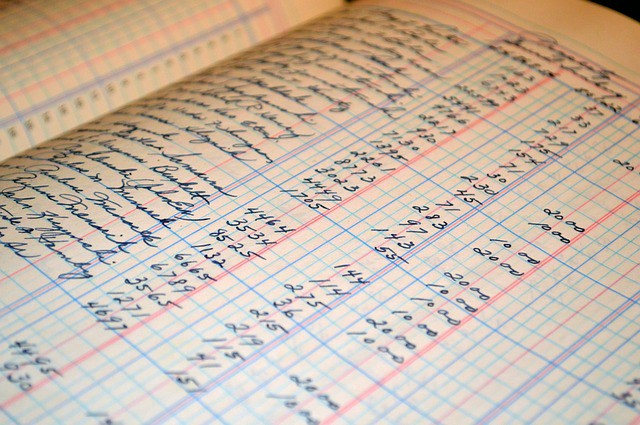
\includegraphics[scale = 0.7]{imgs/account.jpeg}

In account model, it is saved the address and the balance of each address.
For example, the data struct will look like this [(0xabc01, 1.01), (0xabc02, 2.02)].
So the address 0xabc01 has 1.01a of balance and the address 0xabc02 has 2.02 of balance.
In this way, it is possible to easily know how much of balance each address has,
but it is not possible to know how they got in this state.

  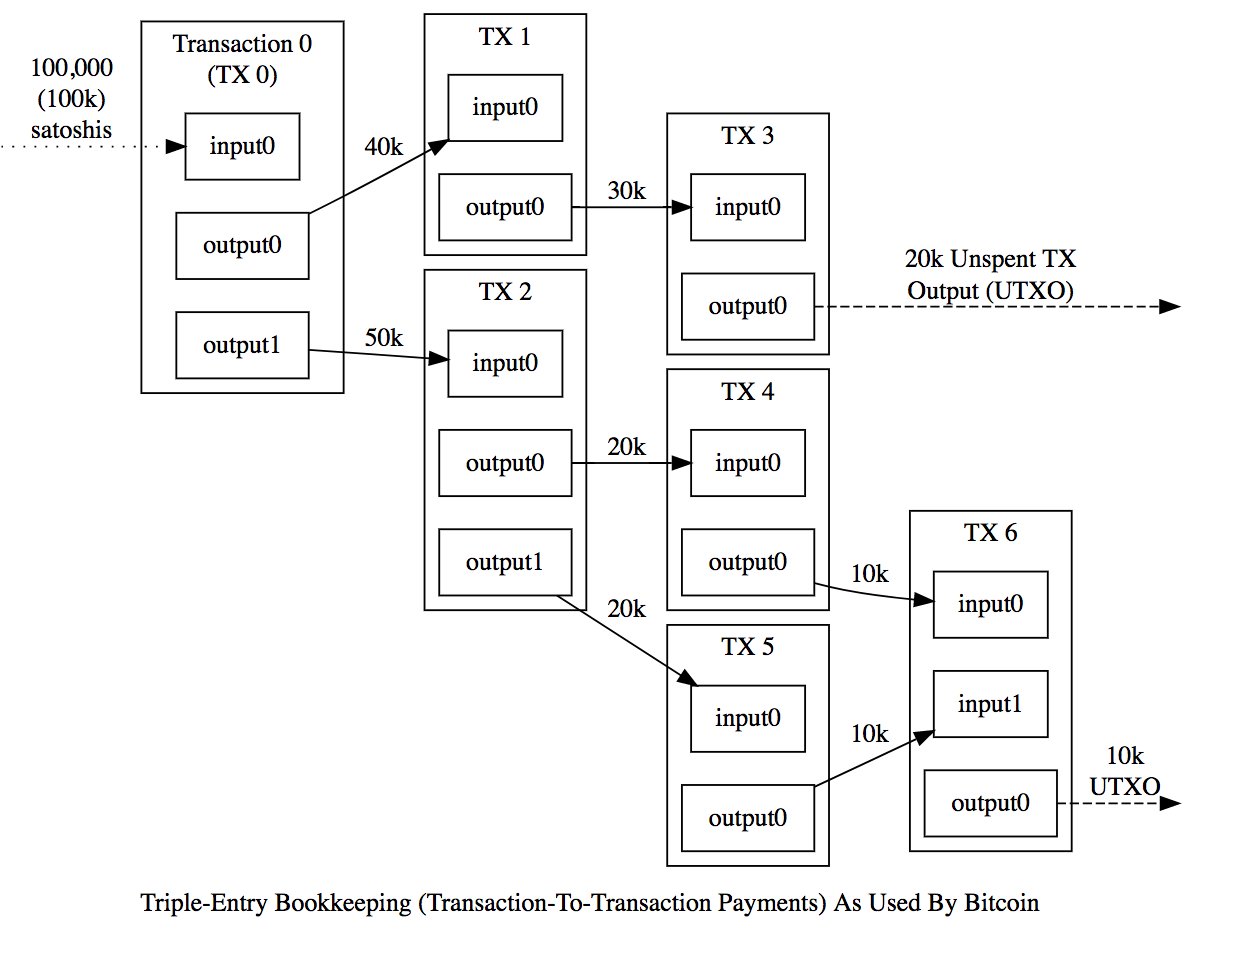
\includegraphics[scale = 0.4]{imgs/utxo.png}

In UTXO model, each transaction is saved in the transaction tree.
Every transaction is composed of multiples inputs and multiples outputs.
But all inputs have to never been spent before.

Because of that, in UTXO model, it is easy to make a new transaction from previous one, but it is harder to know how much each one has.
The wallet that calculate how much balance each address has.

In account model, there could be one kind of vulnerability that is less probabable to happen in UTXO model.
Because there is an undesirable intermediary state that there is some address without balance while another has not already received his money.

For example: \\
bobBalance -= 1 \\
Intermediary State \\
aliceBalance += 1

In account model, it is straight foward to know how much balance each address has.
In UTXO model, this calculation is made offchain. It can be a good thing,
because each user has more privacy.

\subsection{TXTree in Agda}

\section{Methods}

\section{Conclusion}

\newpage
 
\bibliographystyle{apacite}
\bibliography{References}

\end{document}
